\newpage
\section{Problem Formulation}

A company producing injection moulded crates has decided to fully automate its manufacturing process. Currently, three steps in the process are done by humans 1) remove the injection moulded crates from the injection moulding machine 2) de-flash the crates 3) stack crates and remove from the workspace.

The motivation is to both reduce the labour cost and abide by the safety legislation. Figure \ref{fig:manually} shows that the die flash was removed by a labour wearing a mask using a sharp knife. Foul gases from injection moulding machines can cause respiratory diseases. Sharp die flash and the use of sharp tools can easily cause injuries to the hands. These hazards could be eliminated by introducing robotic arms. Meanwhile, robots can operate unceasingly, which could increase production rate.
\begin{figure}[htbp]
   \centering
   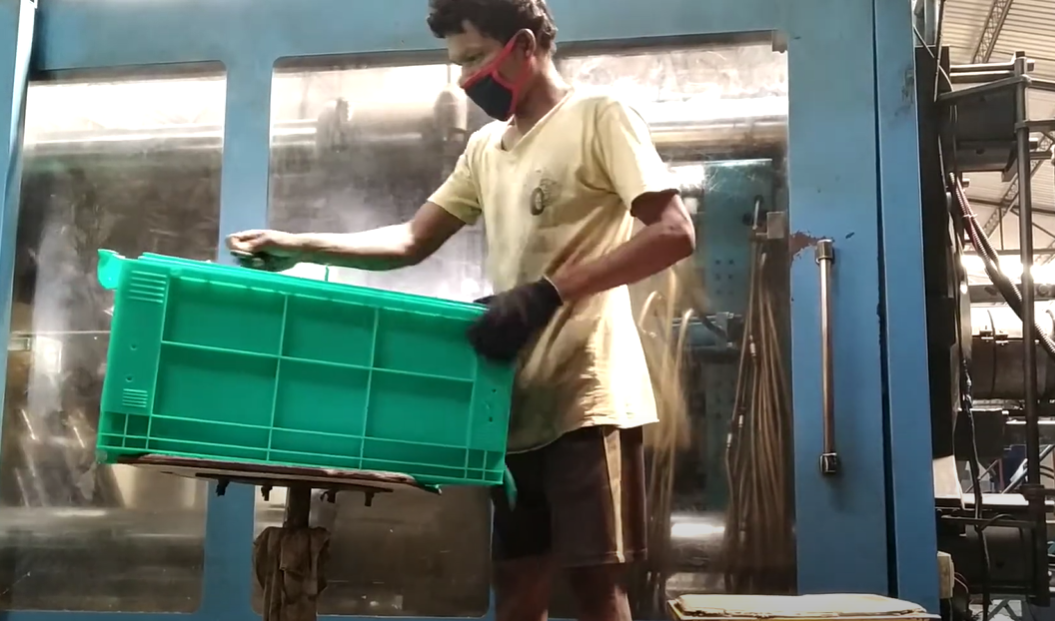
\includegraphics[width=\textwidth]{manually}
   \caption{Screenshot of the injection moulded crates manufacturing process \cite{ref:manually}.}
   \label{fig:manually}
\end{figure}

The company is looking for a complete automation solution that can perform all three tasks with minimal human intervention. The proposed robotic work cell for automating crate production consists of a robotic arm, custom end-of-arm tooling, a die flash removal station, a stacking and transport system, safety equipment, and a control system with custom software. This solution is expected to be efficient, cost-effective, and safe. Although it requires an initial investment and skilled personnel for maintenance, the long-term benefits make it a viable solution for automating the injection moulding process.

\section{Methodology}

The general methodology is illustrated in Figure \ref{fig:stages-of-robotisation}. It's a decision-making process start from suitability analysis. The analysis involves checking the motivation of the company and the robustness of the rest of the system that is not going to be replaced. Next stage is to select the suitable industrial robot and other components of the robot system for the specific task. Then, evaluate the system on both economic and engineering perspective. Iterate the design based on those evaluations. Note that there is no guarantee that this process would yield an optimal or even correct solution.

\begin{figure}[htbp]
   \centering
   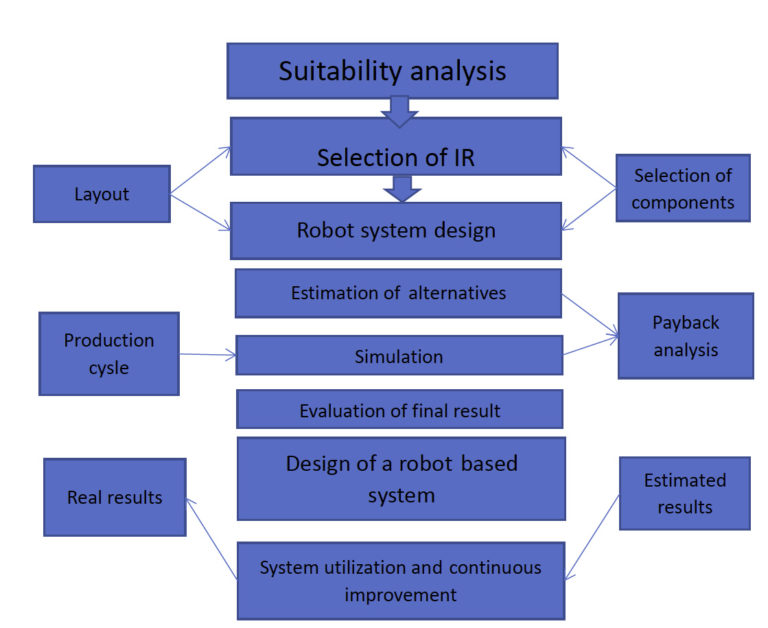
\includegraphics[width=\textwidth]{stages-of-robotisation}
   \caption{Stages of robotisation \cite{ref:robot-cell-design-principles}}
   \label{fig:stages-of-robotisation}
\end{figure}

The design decision of the robot system has been further split into six categories.
\begin{enumerate}[label=(\arabic*), align=left, leftmargin=\parindent, labelwidth=\parindent]
   \item The raw material will be supplied to the injection moulding machine via an automated feeding system ensuring a continuous supply of material and reducing manual intervention.

   \item For the injection moulding process, the company requires reuse the existing injection moulding machine. Upon completion of a crate, a signal will be sent to the control system to initiate the robotic arm's pick-up sequence.

   \item After picking up the crates from the moulding machine, The robotic arm will transport them to the die flash removal station and manoeuvre the crate to cut the die flash.

   \item Once the die flash is removed, the robotic arm will place the finished crates onto a conveyor system for transportation to subsequent stations.

   \item Die flash waste will be handled by the die flash removal station's mechanism to keep the workspace clean and minimising waste-related downtime.

   \item The entire robot cell will be enclosed by a safety fence or barrier with access-controlled gates for authorized personnel only.
\end{enumerate}

The main rationale is minimizing human intervention. Productivity is increased by streamlining material flow. Safety is ensured by various features such as access-control. The health of workers is protected by keeping them away from the workspace. Furthermore, waste control is deployed to reduce downtime for cleaning the workspace.

\section{Design}

\begin{figure}[htbp]
   \centering
   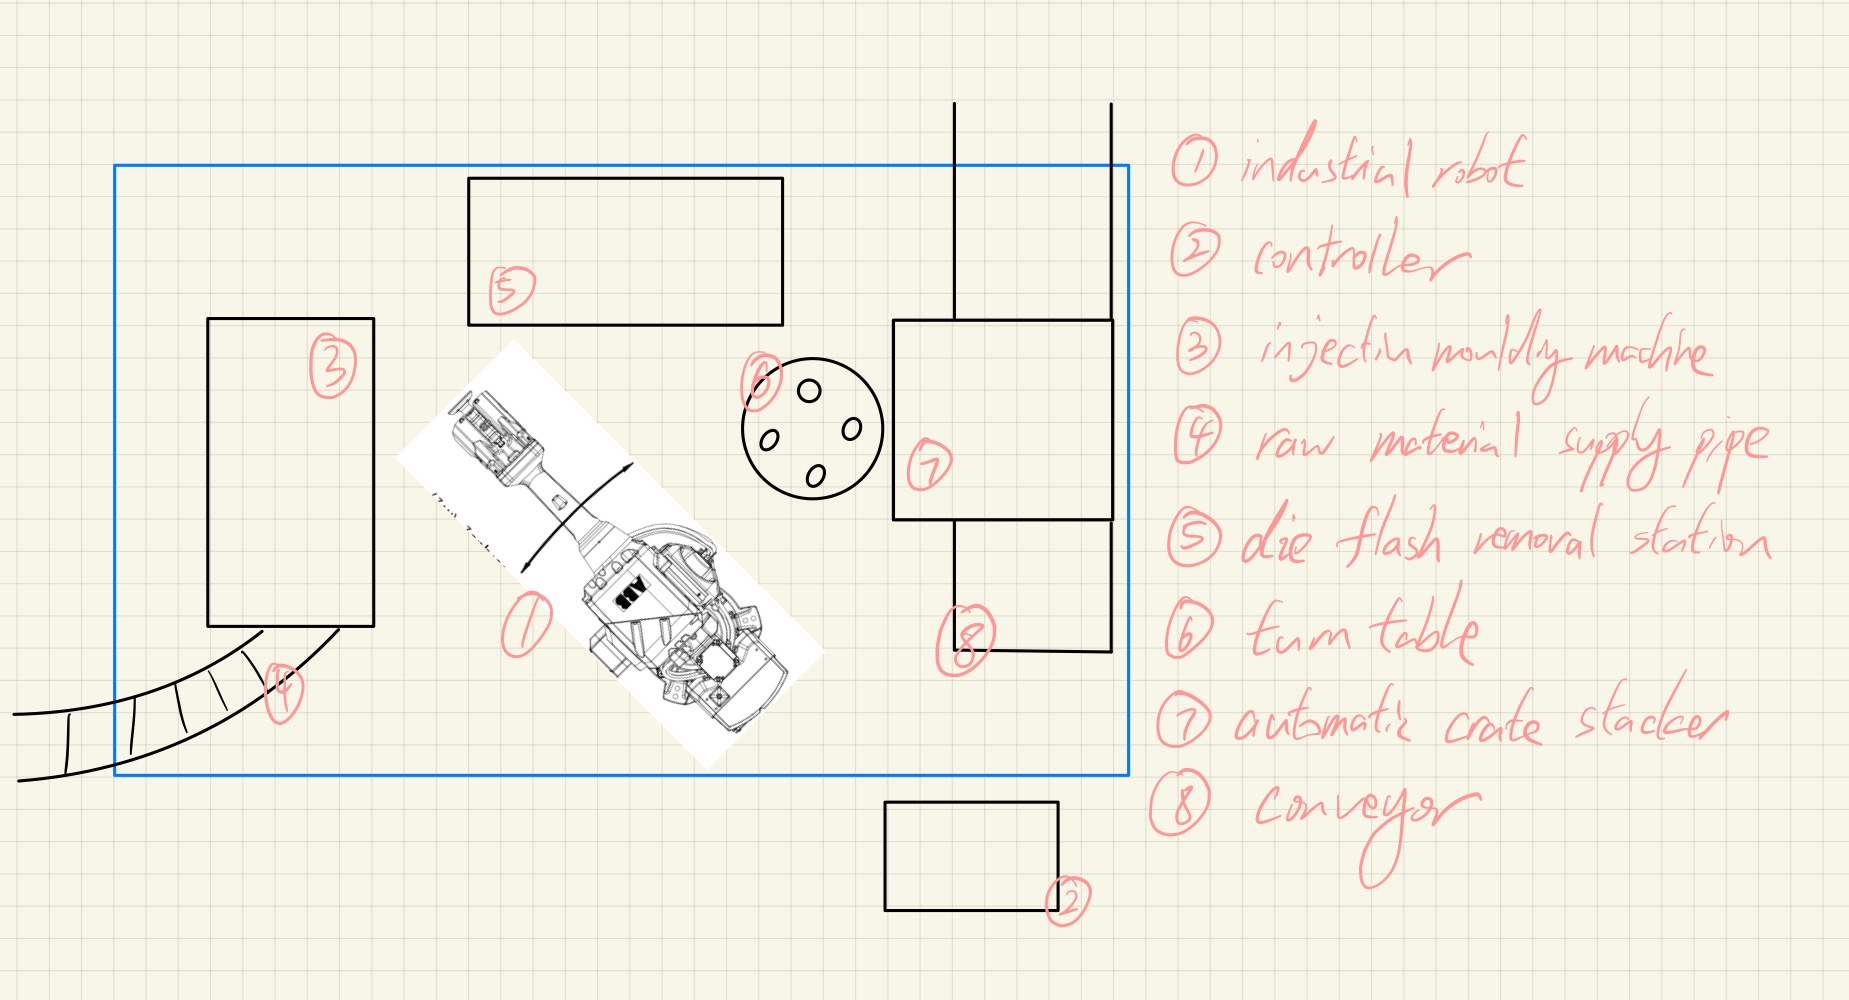
\includegraphics[width=\textwidth]{cell}
   \caption{Sketch of cell design}
   \label{fig:cell}
\end{figure}

Figure \ref{fig:cell} is a top view of the robot work cell demonstrate the rough design for automating the whole production of injection moulding crate. The industrial robot was chosen to be ABB's IRB 4600 which is suitable for compact manufacturing cells. A turntable is place right to the robot was designed to be used to re-grip the crate such that it can be input to the die flash removal station or conveyor in an expected orientation easily. Instead of introducing another robot for stacking and transporting which would consume larger workspace, electricity, and installation and maintenance cost, a simple automatic crate stacker is much preferable. This not only reduces resource consumption, but also greatly reduces the complexity of the system. Programming one robot arm to work is far easier than coordinating two robotic arms.

The planned workflow is as follows: Firstly, the robot will retrieve the crate from the injection moulding machine. After processing one side of the crate at the die flash removal station, it will be placed on the turntable to adjust its position, and then the other side will be processed at the station. Once the flash is removed, the crate orientation will be adjusted on the turntable and placed on the conveyor. The conveyor will transport the crate to the automatic crate stacker for stacking, and finally it will be sent out of the work cell.

\section{Limitations and Improvements}

Despite the proposed automation solution providing numerous benefits, there are still some limitations and areas for improvement.

The initial investment required for implementing the robotic work cell can be high, especially for small and medium-sized companies. The cost of robotic arms and other components, along with installation and integration, can be a significant financial burden.

The successful implementation of the robotic work cell will depend on its seamless integration with the existing injection moulding machine. Potential improvements include better software-level interfacing to ensure smooth coordination between the robot and the injection moulding machine.

The die flash waste collected by the station will still need to be disposed by human workers. One solution is to deploy several automated guided vehicles for empty the bin of each work cell periodically.

\section{Conclusion}

In conclusion, this project proposes a rough automation solution for the injection moulded crate manufacturing process, addressing the company's need to reduce labour costs, increase productivity, comply with safety regulations, and protect the health of workers. Despite initial investment and integration challenges, the long-term benefits make it a viable option for companies looking to improve their processes. Future improvements can be made in improving the interfacing of the existing system and waste disposal.
